\chapter{Project structure}


\section{Introduction}

AVDTA is organized around \textit{projects}. A project is best thought of as a specific scenario under study. For instance, a project might represent a certain demand scenario or network configuration for a city network or subnetwork. The AVDTA GUI contains methods to modify project options, such as link types or intersection controls. Data files can also be copied to and from Excel for easy modification.

\section{GUI}

The AVDTA GUI is designed to interact with projects. Each instance of AVDTA can have a single project open at a time. Projects can be created and opened via the ``File'' menu.

\begin{center}
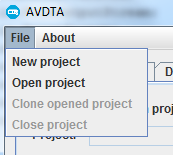
\includegraphics[scale=1]{images/project1.png}
\end{center}


\subsection{New project}
\label{sec:newproject}
To create a new project, you will first be asked to select the root folder. By default, this folder is \texttt{avdta/projects}, but it may be changed.

\begin{center}
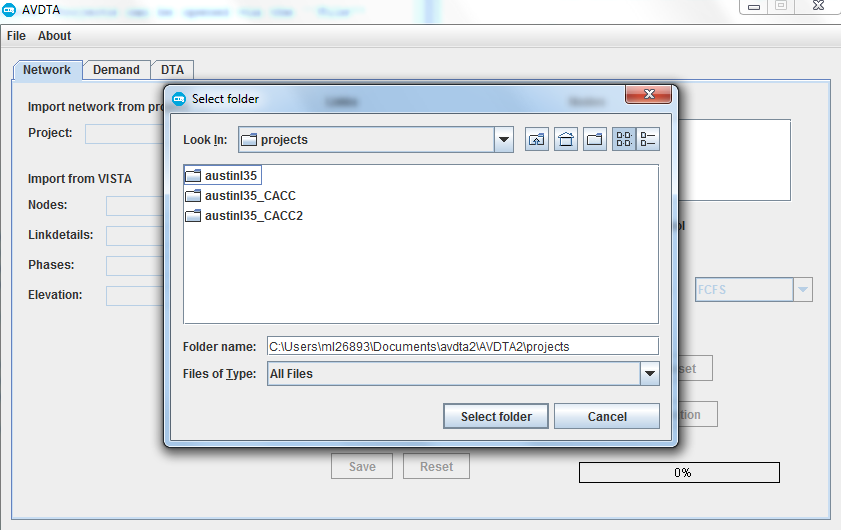
\includegraphics[width=0.8\textwidth]{images/project2.png}
\end{center}

You will then be asked to enter the name of the new project. A project folder with the entered name will be created in the selected root folder.


\begin{center}
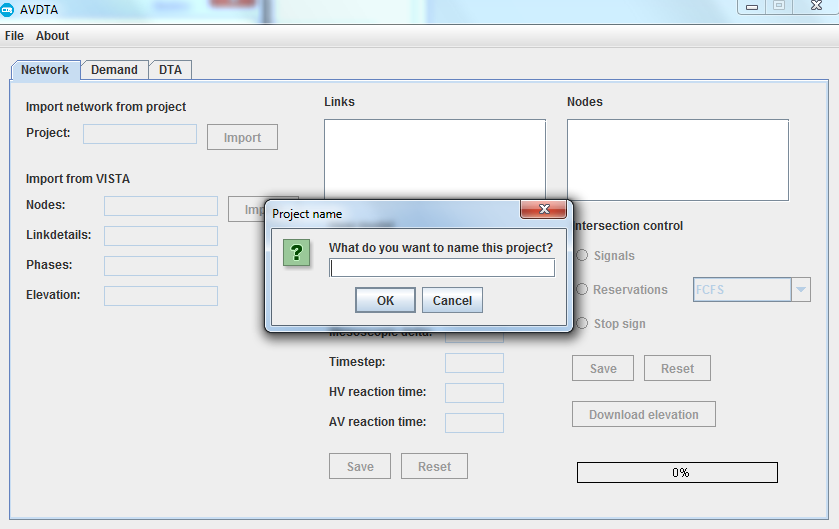
\includegraphics[width=0.8\textwidth]{images/project3.png}
\end{center}

\subsection{Open project}

AVDTA project folders are shown with a special icon. Select a project folder and click ``open project'' to open it.

\begin{center}
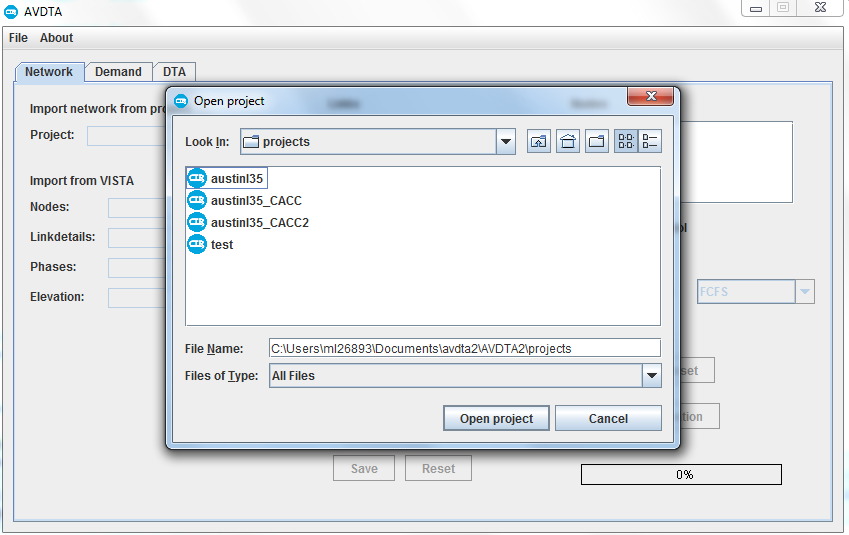
\includegraphics[width=0.8\textwidth]{images/project4.png}
\end{center}

\subsection{Clone opened project}

If a project is open, the AVDTA GUI enables the option of creating a clone. Follow the instructions in Section \ref{sec:newproject} to choose the location and name of the clone. You can also create a copy of a project folder within the file system.

\section{Files and folders}

A project consists of a file folder containing several specific files and subfolders. The project folder, along with many of its files and subfolders, is automatically generated when a new project is created. However, many files will be empty, requiring the import of data from other projects or other sources. Note that removal or modification of these files outside of the AVDTA GUI could result in errors when loading the project. However, adding files or folders will not affect the project. 

Projects contain several types of files. Text files (\texttt{.txt}) contain project inputs or outputs and are intended to be read or modified. However, if modifying these files, ensure that the format and units are correct. Text files are tab-delimited, and have a header indicating the data in each column. Text files may be copied to and from Excel.

Data files (\texttt{.dat}) are used to load the project and are not intended to be opened or modified. Similarly, files with other unknown extensions are not intended to be opened.

\subsection{Files}

\subsubsection{\texttt{project.txt}}
The \texttt{project.txt} file contains project properties used to load the project within AVDTA. The file consists of two columns:
 The file consists of two columns:
\begin{center}
\begin{tabular}{cc}
\hline
key & value\\\hline
\end{tabular}
\end{center}


\paragraph*{name}
This is the project name that is displayed when AVDTA loads a project. This does not have to correspond to the project folder name.

\paragraph*{seed}
This is the random number generator seed. If two projects have matching seeds, actions involving random numbers performed in the same order should have identical outputs.

\paragraph*{type}
This denotes the project type.


\subsubsection{\texttt{options.txt}}
\label{sec:options}

The \texttt{options.txt} file contains project parameters that define the loading and simulation of the project. The file consists of two columns:
\begin{center}
\begin{tabular}{cc}
\hline
key & value\\\hline
\end{tabular}
\end{center}
Keys are case insensitive. Values are a string that could represent multiple data types, such as integers, floating-point numbers, or booleans (``true'' or ``false''). The options file is automatically generated with default values when a project is created. 

\paragraph*{av-reaction-time}
This is used to determine the capacity and congested wave speed increase due to autonomous vehicles when using the multiclass CTM~\cite{levin2016multiclass}. A typical value is 0.5 (s). Note that capacity and congested wave speed are scaled from the values in the \texttt{networks/links.txt} file.

\paragraph*{hv-reaction-time}
This is used to determine the baseline capacity and congested wave speed when using the multiclass CTM~\cite{levin2016multiclass}. A typical value is 1 (s). Note that capacity and congested wave speed are scaled from the values in the \texttt{networks/links.txt} file.

\paragraph*{dynamic-lane-reversal}
If set to ``true'', DLR will be activated on DLR links. DLR is a specific type of CTM link, and the type of links can be set in the \texttt{networks/links.txt} file.

\paragraph*{hvs-use-reservations}
If set to ``true'', HVs will not avoid reservation-controlled intersections in their route choices. Reservations will use the legacy early method for intelligent traffic management~\cite{conde2013intelligent}, adapted to DNL~\cite{levin2016multiclass} for HVs. Otherwise, HVs will avoid reservations in their route choices, passing through reservations only if no other route is available.

\paragraph*{simulation-duration}
This is the duration of the simulation, in seconds. The duration should be sufficiently longer than the demand departure times interval to allow all vehicles to exit the network.

\paragraph*{simulation-mesoscopic-step}
This is the time step used in simulation. For CTM, a typical value is 6 (s). For LTM, a typical value is 10 (s).

\paragraph*{ast-duration}
This the interval for averaging travel times for calculating shortest paths. A typical value is 900 (s).













